\documentclass{minimal}
\usepackage[T1]{fontenc}
\usepackage{newtxtext}
\usepackage{newtxmath}
\usepackage{tikz}
\usetikzlibrary{arrows.meta,calc,positioning}

\pdfpagewidth=1000pt
\pdfpageheight=230pt
\setlength{\paperwidth}{1000pt}
\setlength{\paperheight}{230pt}
\setlength{\textwidth}{1000pt}
\setlength{\textheight}{230pt}
\setlength{\oddsidemargin}{-72pt}
\setlength{\topmargin}{-72pt}
\setlength{\headheight}{0pt}
\setlength{\headsep}{0pt}
\setlength{\footskip}{0pt}
\setlength{\parindent}{0pt}
\pagestyle{empty}

\begin{document}
\begin{tikzpicture}[x=1pt,y=1pt,font=\rmfamily,line cap=round,line join=round]
\tikzset{
  inference/.style={
    -{Latex[length=9pt,width=6pt]},
    draw=black,
    line width=2.2pt
  },
  training/.style={
    -{Latex[length=8pt,width=5pt]},
    draw=black!75,
    densely dashed,
    line width=1.8pt,
    preaction={draw=white,line width=5pt}
  },
  query/.style={
    -{Latex[length=7pt,width=5pt]},
    draw=black!58,
    densely dotted,
    line width=1.6pt
  },
  module/.style={
    rounded corners=8pt,
    draw=black,
    line width=1.55pt,
    fill=white,
    align=center,
    minimum height=48pt,
    inner sep=7pt
  },
  inputbox/.style={module,fill=black!4},
  contextbox/.style={module,fill=black!2},
  statebox/.style={module,fill=black!9},
  transitionbox/.style={module,fill=black!14,line width=2.0pt},
  outputbox/.style={module,fill=black!5},
  chip/.style={
    rounded corners=7pt,
    draw=black!72,
    line width=1.25pt,
    fill=white,
    align=center,
    minimum height=27pt,
    inner sep=5pt
  },
  trainbox/.style={
    rounded corners=6pt,
    draw=black!72,
    line width=1.3pt,
    fill=white,
    align=center,
    minimum height=34pt,
    inner sep=5pt
  },
  lossbox/.style={
    rounded corners=7pt,
    draw=black,
    line width=1.45pt,
    fill=black!7,
    align=center,
    minimum height=34pt,
    inner sep=5pt
  },
  testpanel/.style={
    rounded corners=9pt,
    draw=black!70,
    line width=1.35pt,
    fill=black!2
  },
  optionalpanel/.style={
    rounded corners=9pt,
    draw=black!48,
    densely dashed,
    line width=1.35pt,
    fill=black!7
  },
  testnode/.style={
    rounded corners=5pt,
    draw=black!68,
    line width=1.15pt,
    fill=white,
    align=center,
    minimum height=27pt,
    inner sep=4pt
  }
}

\useasboundingbox (0,0) rectangle (1000,230);
\fill[white] (0,0) rectangle (1000,230);

% One checkpoint and one post-training query bus.
\node[contextbox,minimum width=164pt,minimum height=35pt,
      font=\rmfamily\bfseries\fontsize{18}{21}\selectfont]
  (checkpoint) at (102,211) {same frozen checkpoint};
\draw[query] (checkpoint.east) -- (969,211);
\foreach \x in {119,366,665,907} {
  \draw[query] (\x,211) -- (\x,190);
}
\node[anchor=east,text=black!58,font=\rmfamily\fontsize{18}{21}\selectfont]
  at (978,224) {post-training; no retraining};

% Q1.
\draw[testpanel] (14,15) rectangle (225,190);
\node[anchor=west,font=\rmfamily\bfseries\fontsize{20}{23}\selectfont]
  at (27,172) {A \quad Q1 Forecast skill};
\node[testnode,minimum width=86pt,
      font=\rmfamily\bfseries\fontsize{18}{21}\selectfont]
  (q1terra) at (70,125) {TerraState};
\node[testnode,minimum width=103pt,
      font=\rmfamily\bfseries\fontsize{18}{21}\selectfont]
  (q1base) at (169,125) {matched\\backbone};
\node[testnode,minimum width=166pt,minimum height=42pt,
      font=\rmfamily\bfseries\fontsize{18}{21}\selectfont]
  (q1metric) at (119,64) {paired local metrics\\
  \normalfont\fontsize{18}{21}\selectfont fixed protocol};
\draw[query] (q1terra.south) -- ($(q1metric.north)+(-38pt,0)$);
\draw[query] (q1base.south) -- ($(q1metric.north)+(38pt,0)$);
\node[font=\rmfamily\fontsize{18}{21}\selectfont,text=black!60]
  at (119,29) {Reported rows: Table 1};

% Q2.
\draw[testpanel] (239,15) rectangle (501,190);
\node[anchor=west,font=\rmfamily\bfseries\fontsize{20}{23}\selectfont]
  at (252,172) {B \quad Q2 Load-bearing};
\node[testnode,minimum width=127pt,
      font=\rmfamily\bfseries\fontsize{18}{21}\selectfont]
  (full) at (316,132) {full};
\node[testnode,minimum width=127pt,line width=1.7pt,
      font=\rmfamily\bfseries\fontsize{18}{21}\selectfont]
  (closurecut) at (316,94) {closure cut $r_h=0$};
\node[testnode,minimum width=127pt,densely dashed,draw=black!50,
      font=\rmfamily\bfseries\fontsize{18}{21}\selectfont]
  (tid) at (316,56) {support: $T\!\to I$};
\node[testnode,minimum width=77pt,minimum height=102pt,
      font=\rmfamily\bfseries\fontsize{18}{21}\selectfont]
  (endpoint) at (443,94) {paired\\endpoint\\effect};
\draw[query] (full.east) -- ($(endpoint.west)+(0,38pt)$);
\draw[query] (closurecut.east) -- (endpoint.west);
\draw[query] (tid.east) -- ($(endpoint.west)+(0,-38pt)$);
\node[font=\rmfamily\fontsize{18}{21}\selectfont,text=black!60]
  at (370,28) {same samples, weights, prior};

% Q3.
\draw[testpanel] (515,15) rectangle (817,190);
\node[anchor=west,font=\rmfamily\bfseries\fontsize{20}{23}\selectfont]
  at (528,172) {C \quad Q3 Driver response};
\node[font=\rmfamily\fontsize{18}{21}\selectfont,text=black!62]
  at (666,148) {future weather $\rightarrow T_\psi$ only};
\node[testnode,minimum width=78pt,
      font=\rmfamily\bfseries\fontsize{18}{21}\selectfont]
  (actual) at (564,119) {actual};
\node[testnode,minimum width=78pt,
      font=\rmfamily\bfseries\fontsize{18}{21}\selectfont]
  (mean) at (666,119) {mean};
\node[testnode,minimum width=90pt,
      font=\rmfamily\bfseries\fontsize{18}{21}\selectfont]
  (donor) at (765,119) {matched donor};
\node[testnode,minimum width=236pt,minimum height=35pt,
      font=\rmfamily\bfseries\fontsize{18}{21}\selectfont]
  (q3readout) at (666,77) {state \(\cdot\) output \(\cdot\) score};
\draw[query] (actual.south) -- ($(q3readout.north)+(-68pt,0)$);
\draw[query] (mean.south) -- (q3readout.north);
\draw[query] (donor.south) -- ($(q3readout.north)+(68pt,0)$);
\node[testnode,minimum width=256pt,minimum height=42pt,densely dashed,
      draw=black!48,fill=black!7,
      align=center,font=\rmfamily\bfseries\fontsize{18}{21}\selectfont]
  at (666,38) {pre-registered stratum:\\hot-dry vs matched-normal};

% Q4 is visually and spatially downgraded.
\draw[optionalpanel] (831,15) rectangle (986,190);
\node[anchor=west,text=black!58,
      font=\rmfamily\bfseries\fontsize{19}{22}\selectfont]
  at (844,172) {D \quad Q4 Optional};
\node[testnode,densely dashed,draw=black!48,minimum width=116pt,
      font=\rmfamily\bfseries\fontsize{18}{21}\selectfont]
  (direct) at (908,132) {direct};
\node[testnode,densely dashed,draw=black!48,minimum width=116pt,
      font=\rmfamily\bfseries\fontsize{18}{21}\selectfont]
  (composed) at (908,96) {composed};
\node[testnode,densely dashed,draw=black!48,minimum width=126pt,
      minimum height=48pt,
      text width=116pt,
      align=center,font=\rmfamily\bfseries\fontsize{18}{21}\selectfont]
  (guards) at (908,48) {endpoint guard +\\non-collapse};
\draw[query] (direct.south) -- ($(guards.north)+(-27pt,0)$);
\draw[query] (composed.south) -- ($(guards.north)+(27pt,0)$);

\end{tikzpicture}
\end{document}
